\section{Image Cartooning} % (fold)
\label{sec:image_cartooning}
    
    In this section we present a technique to turn an input image $g$ into a cartooned image $u$. For this we will make use of the ROF Model, TVL1 Model and most of all the real-time minimizer for the Mumford-Shah Function, presented in section \ref{sec:the_mumford_shah_functional}. Using the model of Rudin, Osher and Fatemi and the TVL1 Model meant for us to find the right parameter $\lambda$ to smooth the image enough, but still preserve edges. We will exchange the data fidelity term $G$, by another term $G^{q}_{\gamma}$. This leads to a nice cartoon representation of our image. For this, we first propose the new data fidelity term and then we compute the corresponding proximity operator, which depends on the function $G^{q}_{\gamma}$.

    \subsection{A new data fidelity term} % (fold)
    \label{sub:a_new_data_fidelity_term}

        Recalling the Mumford-Shah energy function we had
            $$
                E_{MS}(u) = ||u - g||_{2}^{2} + \sum_{i = 1}^{N} \sum_{j = 1}^{M} \min(\lambda |(\nabla u)_{i,j}|, \nu),
            $$
        where we set the data fidelity term to $G(u) = ||u - g||_{2}^{2}$. The idea for cartooning is now to replace $G$ with a function $G^{q}_{\gamma}$ defined by
            \begin{equation}
                G^{q}_{\gamma}(u) := ||u - g||_{2}^{2} + \gamma ||u - u^{\textnormal{prev}}||_{q}^{q}.
                \label{eq:ms_new_regularizer}
            \end{equation}
        Here, $u^{\textnormal{prev}}$ is the $u$, which was obtained in the previous iteration, hence the notation. The additional $l_{q}$ regularization aims to handle the tradeoff between the current and the previous estimate of $u$. It forces $u$ not to change too much during the iterations process. But as mentioned above, we need to compute the proximity operator with respect to the new function $G^{q}_{\gamma}$. Using again \ref{eq:proximity_operator_reloaded}, we obtain

            \begin{equation}
                u = (\textnormal{Id} + \tau \partial G^{q}_{\gamma})^{-1}(\tilde{u}) = \arg \min_{u \in X} \frac{||u - \tilde{u}||_{2}^{2}}{2} + \tau \left( ||u - g||_{2}^{2} + \gamma ||u - u^{\textnormal{prev}}||_{q}^{q} \right).
                \label{eq:prox_new_data_fidelity_term}
            \end{equation}

        As one can see, the new proximity operator is dependent on how the norm in the additional term is chosen. We are looking at the cases where we have $q = 1$ and $q = 2$. In the appendix of \cite{Strekalovskiy-Cremers-eccv14} they suggest using $q = 1.5$ and therefore also compute the proximal operator. In our tests, this did not have that big impact, for that we choose to use the $l_{1}$ and $l_{2}$ norm, respectively.

        Let us first consider the case where $q = 2$. Then we obtain for the proximal operator
            \begin{eqnarray}
                u = (\textnormal{Id} + \tau \partial G^{q}_{\gamma})^{-1}(\tilde{u}) &=& \arg \min_{u \in X} \frac{||u - \tilde{u}||_{2}^{2}}{2} + \tau \left( ||u - g||_{2}^{2} + \gamma ||u - u^{\textnormal{prev}}||_{2}^{2} \right) \notag \\
                &\Longleftrightarrow& 0 \in \partial \bigg( \frac{||u - \tilde{u}||_{2}^{2}}{2} + \tau \left( ||u - g||_{2}^{2} + \gamma ||u - u^{\textnormal{prev}}||_{2}^{2} \right) \bigg)\notag \\
                &\Longleftrightarrow& 0 \in u - \tilde{u} + 2\tau(u - g) + 2\tau\gamma (u - u^{\textnormal{prev}}) \notag \\
                &\Longleftrightarrow& u \big( 1 + 2\tau + 2\tau\gamma \big) = \tilde{u} + 2\tau g + 2\tau\gamma u^{\textnormal{prev}} \notag \\
                &\Longleftrightarrow& u = \frac{\tilde{u} + 2\tau g + 2\tau\gamma u^{\textnormal{prev}}}{1 + 2\tau + 2\tau\gamma} \notag
            \end{eqnarray}
        Overall, we obtain pointwise for all $i = 1, ..., N$ and $j = 1, ..., M$
            \begin{equation}
                u_{i, j} = \frac{\tilde{u}_{i, j} + 2\tau g_{i, j} + 2\tau\gamma u^{\textnormal{prev}_{i, j}}}{1 + 2\tau + 2\tau\gamma}
                \label{eq:prox_d_q_two}
            \end{equation}

        The other option was to set $q = 1$. In this case we obtain the non-differentiable $l_{1}$ norm and we need to make use of the subgradient. We need to do a case analysis. For this, let $y_{i}$ be the subgradient of the term $||u - u^{\textnormal{prev}}||_{1}$ in the i-th component with $y_{i} \in [-1, 1]$. Then we get with the the equations for the proximity operator:
            \begin{eqnarray}
                u = (\textnormal{Id} + \tau \partial G^{q}_{\gamma})^{-1}(\tilde{u}) &=& \arg \min_{u \in X} \frac{||u - \tilde{u}||_{2}^{2}}{2} + \tau \left( ||u - g||_{2}^{2} + \gamma ||u - u^{\textnormal{prev}}||_{1}^{1} \right) \notag \\
                &\Longleftrightarrow& 0 \in \partial \bigg( \frac{||u - \tilde{u}||_{2}^{2}}{2} + \tau \left( ||u - g||_{2}^{2} + \gamma ||u - u^{\textnormal{prev}}||_{1} \right) \bigg)\notag \\
                &\Longleftrightarrow& 0 \in u - \tilde{u} + 2\tau (u - g) + \tau\gamma y \notag
            \end{eqnarray}
        We will look at the i-the row of this equation.
        \begin{enumerate}
            \item Consider the first case and assume that $u_{i} - u^{\textnormal{prev}}_{i} > 0$. Then clearly, $y_{i} = 1$ and
                \begin{eqnarray}
                    0 \in u_{i} - \tilde{u}_{i} + 2\tau (u_{i} - g_{i}) + \tau\gamma &\Longleftrightarrow& u_{i} (1 + 2\tau) = \tilde{u}_{i} + 2\tau g_{i} - \tau\gamma \notag \\
                    &\Longleftrightarrow& u_{i} = \frac{\tilde{u}_{i} + 2\tau g_{i} - \tau\gamma}{1 + 2\tau}. \notag
                \end{eqnarray}
            Then, the last equation implies
                \begin{eqnarray}
                    \frac{\tilde{u}_{i} + 2\tau g_{i} - \tau\gamma}{1 + 2\tau} - u^{\textnormal{prev}} > 0 &\Longleftrightarrow& \tilde{u}_{i} + 2\tau g_{i} - \tau\gamma - u^{\textnormal{prev}} (1 + 2\tau) > 0 \notag \\
                    &\Longleftrightarrow& \tilde{u}_{i} + 2\tau g_{i} - u^{\textnormal{prev}} (1 + 2\tau) > \tau\gamma.
                \end{eqnarray}
            \item Assuming that $u_{i} - u^{\textnormal{prev}}_{i} < 0$ leads to a similar expression, but we need to exchange the sign in front of the term $\tau\gamma$, since in this case it holds that $y_{i} = -1$. Overall, we obtain
                $$
                    u_{i} = \frac{\tilde{u}_{i} + 2\tau g_{i} + \tau\gamma}{1 + 2\tau}.
                $$
            As in 1. we can compute
                \begin{eqnarray}
                    \frac{\tilde{u}_{i} + 2\tau g_{i} + \tau\gamma}{1 + 2\tau} - u^{\textnormal{prev}} < 0 &\Longleftrightarrow& \tilde{u}_{i} + 2\tau g_{i} + \tau\gamma - u^{\textnormal{prev}} (1 + 2\tau) < 0 \notag \\
                    &\Longleftrightarrow& \tilde{u}_{i} + 2\tau g_{i} - u^{\textnormal{prev}} (1 + 2\tau) < -\tau\gamma.
                \end{eqnarray}
            \item In the last case we assume that the equality $u_{i} = u^{\textnormal{prev}}_{i}$ holds. Then we have that $y_{i} \in [-1, 1]$ can be set arbitrary. To show in which case this setting holds we plug $y_{i}$ into the equation, set $u_{i} = u^{\textnormal{prev}}_{i}$ and observe
                \begin{eqnarray}
                    0 \in u^{\textnormal{prev}}_{i} - \tilde{u}_{i} + 2\tau (u^{\textnormal{prev}}_{i} - g_{i}) + \tau\gamma y_{i} &\Longleftrightarrow& u^{\textnormal{prev}}_{i} - \tilde{u}_{i} + 2\tau (u^{\textnormal{prev}}_{i} - g_{i}) = - \tau\gamma y_{i} \notag \\
                    &\Longleftrightarrow& \tilde{u}_{i} - u^{\textnormal{prev}}_{i} (1 + 2\tau) + 2\tau g_{i} = \tau\gamma y_{i} \notag \\
                    &\Longleftrightarrow& |\tilde{u}_{i} - u^{\textnormal{prev}}_{i} (1 + 2\tau) + 2\tau g_{i}| = |\tau\gamma y_{i}| \le \tau \gamma \notag
                \end{eqnarray}
        \end{enumerate}

        Overall, we have the following representation of the proximity operator to this problem:
            \begin{subequations}
                \begin{align}
                    u &= (\textnormal{Id} + \tau\,\partial\,G^{q}_{\gamma})^{-1}(\tilde{u}) \Longleftrightarrow \\
                    u_{i, j} &=
                        \begin{dcases*}
                            \frac{\tilde{u}_{i,j} + 2\tau g_{i,j} - \tau\gamma}{1 + 2\tau} & \textnormal{if\, $\tilde{u}_{i,j} + 2\tau g_{i,j} - u^{\textnormal{prev}} (1 + 2\tau) > \tau\gamma$,} \\
                            \frac{\tilde{u}_{i,j} + 2\tau g_{i,j} + \tau\gamma}{1 + 2\tau} & \textnormal{if\, $\tilde{u}_{i,j} + 2\tau g_{i,j} - u^{\textnormal{prev}} (1 + 2\tau) < -\tau\gamma$,} \\
                            u^{\textnormal{prev}}_{i,j} & \textnormal{if\, $|\tilde{u}_{i,j} - u^{\textnormal{prev}}_{i,j} (1 + 2\tau) + 2\tau g_{i,j}| \le \tau\gamma$},
                        \end{dcases*}
                \label{eq:prox_d_q_one}
                \end{align}
            \end{subequations}
        for all $i = 1, ..., N$, $j = 1, ..., M$.

    % subsection a_new_data_fidelity_term (end)

    \subsection{Edge Highlighting} % (fold)
    \label{sub:edge_highlighting}
        
        Another idea Strekalovskiy and Cremers proposed in \cite{Strekalovskiy-Cremers-eccv14} was to use the edge set $K_{MS}$ in order to highlight edges in the smoothed images.

        Assume that $x \in K_{MS}$ then we have $|\nabla u(x)| \ge \sqrt{\frac{\nu}{\lambda}}$ by definition. This notation is equivalent to setting
            $$
                \frac{|\nabla u(x)|}{\sqrt{\frac{\nu}{\lambda}}} \ge 1.
            $$
        Further, we have by discretizing the operator $\nabla$ with forward differences that
            $$
                |\nabla u(x)| = \max_{|u(x)| \le 1} |\nabla u(x)| = \max_{|x| \le 1} |\frac{u(x+\delta x) - u(x)}{\delta x}|.
            $$
        This means we have $|\nabla u(x)| \le \sqrt{2}$ and for that
            $$
                1 \le \frac{|\nabla u(x)|}{\sqrt{\frac{\nu}{\lambda}}} \le \frac{\sqrt{2}}{\sqrt{\frac{\nu}{\lambda}}}.
            $$
        Applying the logarithm to each of the terms we get
            $$
                0 \le \log \bigg( \frac{|\nabla u(x)|}{\sqrt{\frac{\nu}{\lambda}}} \bigg) \le \log \bigg( \frac{\sqrt{2}}{\sqrt{\frac{\nu}{\lambda}}} \bigg).
            $$
        If we now divide each term by the last one, we observe
            $$
                0 \le \frac{\log \bigg( \frac{|\nabla u(x)|}{\sqrt{\frac{\nu}{\lambda}}} \bigg)}{\log \bigg( \frac{\sqrt{2}}{\sqrt{\frac{\nu}{\lambda}}} \bigg)} \le 1.
            $$
        With these calculations, we now define a $v \in [0, 1]$ by
            $$
                v := \frac{\log \bigg( \frac{|\nabla u(x)|}{\sqrt{\frac{\nu}{\lambda}}} \bigg)}{\log \bigg( \frac{\sqrt{2}}{\sqrt{\frac{\nu}{\lambda}}} \bigg)},
            $$
        then, since $\nu$ and $\lambda$ are constant values, this parameter $v$ only increases if $|\nabla u(x)|$ increases and decreases if $|\nabla u(x)|$ decreases. For this reason $v$ can serve as an edge indicator. Then the idea proposed by \cite{Strekalovskiy-Cremers-eccv14} is to multiply each RGB value $u(x)$ by
            $$
                1 - v \in [0, 1],
            $$
        if $x \in K_{MS}$. On the other hand, if $x \notin K_{MS}$ the value $u(x)$ will not be changed. Then points in the imaged domain $\Omega$ with strong edges are painted darker, as those where we do not find edges.

    % subsection edge_highlighting (end)

    \subsection{Image Comparison} % (fold)
    \label{sub:image_comparison}

        In this subsection we want to present solutions of the three models: ROF, TVL1 and real-time Mumford-Shah minimizer. We will compare run-time of the models - on a CPU and GPU - and provide the best estimations for the parameters $\lambda, \nu$ and $\gamma$. We start with the ROF Model:

        \begin{figure}[ht]
            \centering
            \begin{subfigure}[b]{0.45\textwidth}
                \includegraphics[width=\textwidth]{img/cartooning/rof/001hepburn.png}
                \caption{$\lambda = 0.01$}
            \end{subfigure}
            \begin{subfigure}[b]{0.45\textwidth}
                \includegraphics[width=\textwidth]{img/cartooning/tvl1/035hepburn.png}
                \caption{$\lambda = 0.35$}
            \end{subfigure}
            \caption[Cartooning Comparison of Hepburn using ROF and TVL1]{Comparison of cartooning applying the ROF Model (left) and the TVL1 Model (right) to the Audrey Hepburn image}
        \label{fig:cartooning_comparison_hepburn}
        \end{figure}

        \begin{figure}[ht]
            \centering
            \begin{subfigure}[b]{0.45\textwidth}
                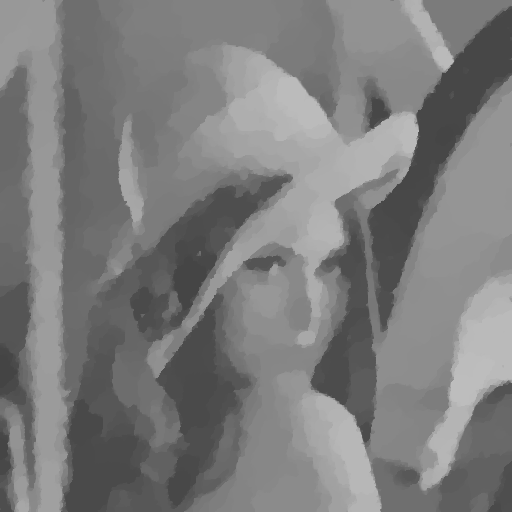
\includegraphics[width=\textwidth]{img/cartooning/rof/001lena.png}
                \caption{$\lambda = 0.01$}
            \end{subfigure}
            \begin{subfigure}[b]{0.45\textwidth}
                \includegraphics[width=\textwidth]{img/cartooning/tvl1/035lena.png}
                \caption{$\lambda = 0.35$}
            \end{subfigure}
            \caption[Cartooning Comparison of Lena using ROF and TVL1]{Comparison of cartooning applying the ROF Model (left) and the TVL1 Model (right) to the Lena image}
        \label{fig:cartooning_comparison_lena}
        \end{figure}

        One can see that the difference of these two models becomes visible at the edges. As the ROF Model really smoothes the image and provides pretty good cartooned images, the TVL1 Model preserves more edges and details in the images. But, what both models have in common: the cartoon images do not fit the imagination one has when thinking about cartoons. Therefore, we not only applied the real-time minimzer for the Mumford-Shah model to the images, we also made use of the above data fidelity term $G^{q}_{\gamma}$ and the method for edge highlighting. We start with $q = 1$.

        \begin{figure}[ht]
            \centering
            \begin{subfigure}[b]{0.45\textwidth}
                \includegraphics[width=\textwidth]{img/cartooning/realtime/104hepburn500.png}
                \caption{$\alpha = 500, \lambda = 0.4, \gamma = 1$}
            \end{subfigure}
            \begin{subfigure}[b]{0.45\textwidth}
                \includegraphics[width=\textwidth]{img/cartooning/realtime/1004hepburn500.png}
                \caption{$\alpha = 500, \lambda = 0.4, \gamma = 10$}
            \end{subfigure}
            \begin{subfigure}[b]{0.45\textwidth}
                \includegraphics[width=\textwidth]{img/cartooning/realtime/2004hepburn500.png}
                \caption{$\alpha = 500, \lambda = 0.4, \gamma = 20$}
            \end{subfigure}
            \begin{subfigure}[b]{0.45\textwidth}
                \includegraphics[width=\textwidth]{img/cartooning/realtime/5005hepburn500.png}
                \caption{$\alpha = 500, \lambda = 0.5, \gamma = 50$}
            \end{subfigure}
            \caption{Cartooning of.}
        \label{fig:cartooning_hepburn_realtime}
        \end{figure}

        By estimating the best fits for our parameters we ran a huge amount of tests. Using the framework presented for the Mumford-Shah Model, we observed a lot of possible images and chose the ones, which fitted best for us. Finding nicely cartooned images for the ROF and TVL1 Model, respectively, was a harder task. We obtained also a large number of images, but only a few fitted to be considered as cartoon images. Overall, the real-time minimizer is the model to choose, if one seeks for cartooned images or movies.

    \subsection{Computational Comparison} % (fold)
    \label{sub:computational_comparison}
        
        In this part of the section we present the run-times for the three models for the best fitted parameters for cartooning. We also provide the best time-step parameter $\tau$ for the ROF and TVL1 model, the iterations to convergence and the final (minimal) energy of the model. Further, we discuss some implementation issues and the comparison of running the algorithms on a CPU and GPU.

        For this computational comparison we use the Audrey Hepburn image with the parameters presented in subsection \ref{sub:image_comparison}. For the Mumford-Shah Model the parameter $\tau$ is set to $0.25$ by definition of th proposed algorithm in section \ref{sec:a_firs_order_primal_dual_algorithm}.
        \begin{center}
            \begin{tabular}{| l | l | l | l | l | l |}
            \hline
            Model & $\tau$ & CPU time & GPU time & Iterations & Energy  \\ \hline
            ROF & 0.25 &  &  &  &  \\ \hline
            ROF & 0.5 &  &  &  &  \\ \hline
            ROF & 0.97 &  &  &  &  \\ \hline
            TVL1 & 0.25 &  &  &  &  \\ \hline
            TVL1 & 0.5 &  &  &  &  \\ \hline
            TVL1 & 0.97 &  &  &  &  \\ \hline
            Mumford-Shah & 0.25 &  &  &  &  \\ \hline
            Mumford-Shah & 0.25 &  &  &  &  \\ \hline
            Mumford-Shah & 0.25 &  &  &  &  \\ \hline
            \end{tabular}
        \end{center}
    % subsection computational_comparison (end)

    % subsection image_comparison (end)

% section image_cartooning (end)